%! Author = Philipp Emmenegger
%! Date = 08/06/2021

\section{Quality}
\begin{enumerate}
    \item Identify Requirements
    \item Define measurable Criteria
    \item Inspect and Adapt
\end{enumerate}

\subsection{Requirements}
\textbf{Functional}
\begin{itemize}
    \item Acquired together with the customer
    \item Usually gathered by a Requirement Engineer
    \item Easy to verify
\end{itemize}
\textbf{Non-functional}
\begin{itemize}
    \item Defined by the customer and the developers
    \item Usually gathered by a Software Architect
    \item Often harder to verify
\end{itemize}

\subsection{Software Aging}
\textbf{Causes}
\begin{itemize}
    \item Lack of movement
    \item Ignorant surgery
\end{itemize}
\textbf{Costs}
\begin{itemize}
    \item Inability to keep up
    \item Reduced performance
    \item Decreasing reliability
\end{itemize}
\textbf{Remedy}
\begin{itemize}
    \item Stop the deterioration
    \item Design for success
    \item Planning ahead
\end{itemize}

\subsection{Quality Measures}
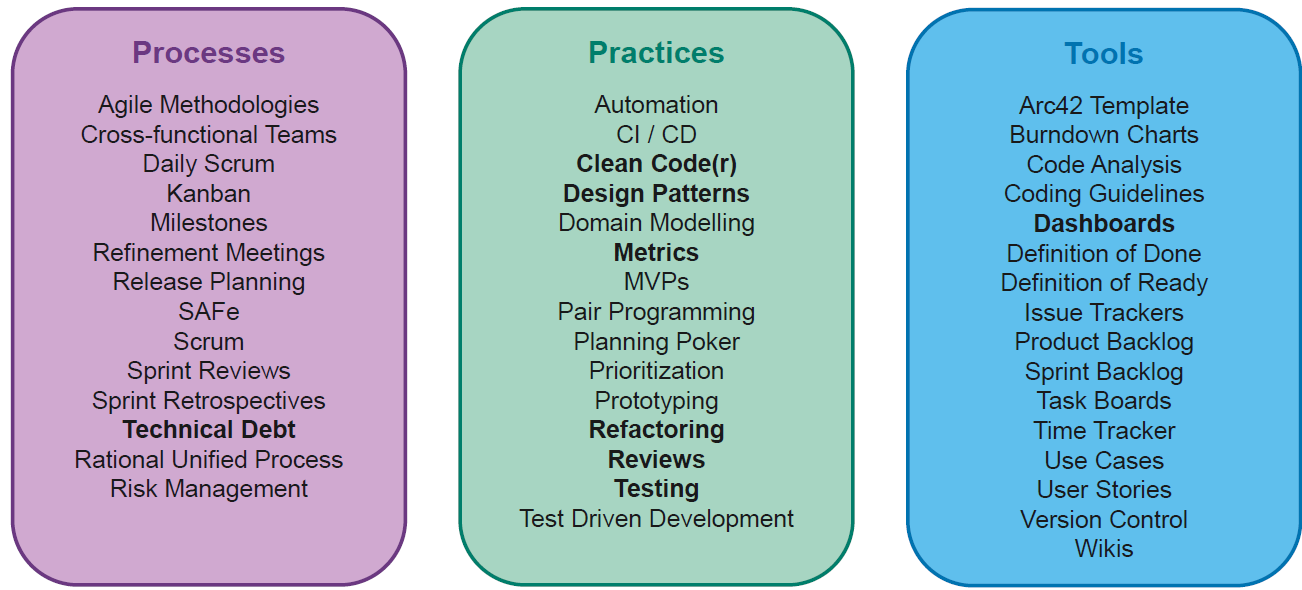
\includegraphics[width=\linewidth]{../img/quality_measures.png}

\subsection{Technical Dept}
\begin{itemize}
    \item Amount of additional rework caused by an easy solution
    \item Not necessary a bad thing
    \item If not repaid, it can grow (interest)
    \item Might not increase linear
\end{itemize}
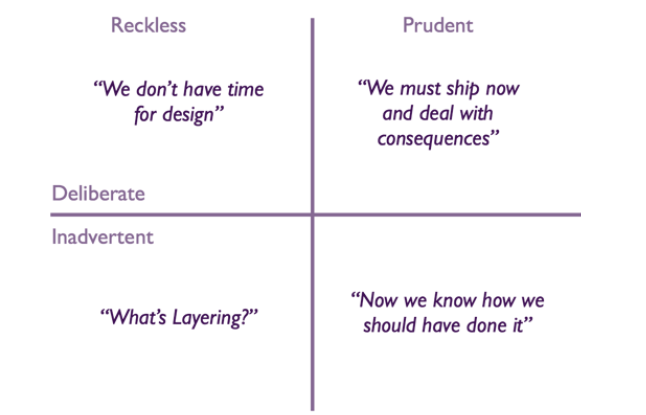
\includegraphics[width=\linewidth]{../img/technical_dept.png}

\subsection{Software Metrics}
\textbf{Product Metrics}
\begin{itemize}
    \item Lines of Code
    \item Code Coverage
    \item Cyclomatic Complexity
\end{itemize}
\textbf{Project Metrics}
\begin{itemize}
    \item Number of Git-Commits
    \item Number of Changed files in Merge-Requests
    \item Number of changes to a file in a time period
\end{itemize}

\subsubsection{Caution}
\begin{itemize}
    \item Only indicators and might be misleading
    \item Acceptable metric does not imply good quality
    \item Choose reasonable scale
    \item Define Actions for unacceptable results
    \item Never use metrics for a reward system
\end{itemize}

\subsubsection{Visualization - Polymetric View}
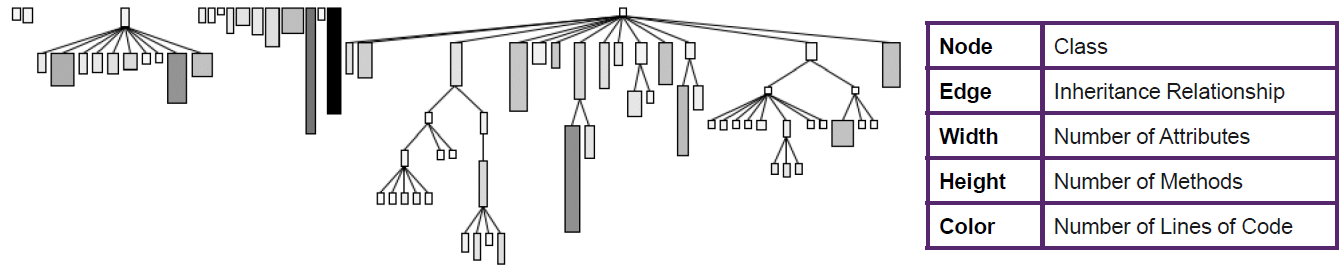
\includegraphics[width=\linewidth]{../img/polymetric_view_1.png}
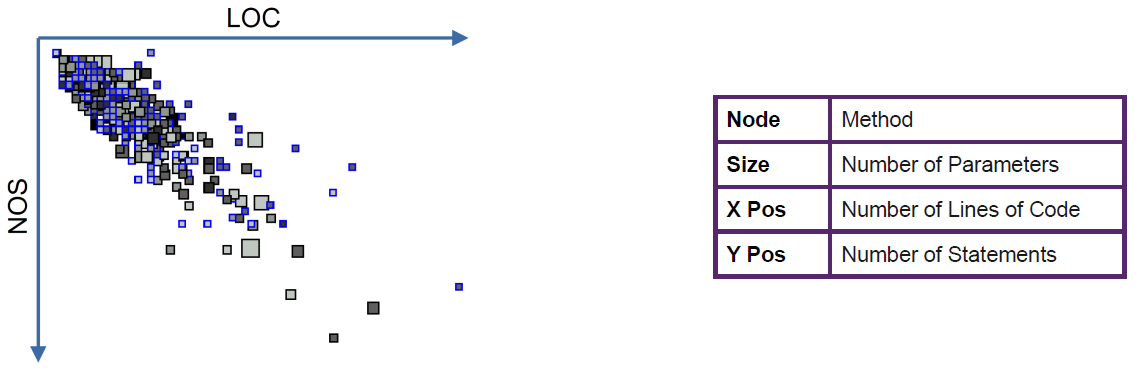
\includegraphics[width=\linewidth]{../img/polymetric_view_2.png}



















